\section{Elektronika tlakové desky}
\label{E4-tlakovka}
Tlaková plocha se díky pružné podložce a~nažehlovací fólii může ve všech směrech naklánět, a~díky tomu se při používání mění vzdálenost od čtyř snímacích
cívek. Tlaková plocha je především terčík, který slouží jako se\-kun\-dár\-ní cívka k~cívce vyleptané v~mědi. LDC1614 pak při měření do snímacích 
cívek pouští frekvenci, která se dá nastavit externím zdrojem na 2-40~MHz nebo použít interní oscilátor, který je nastaven na 40 MHz. 
Na základě Foucaultových proudů se pak dá určit vzdálenost terčíku od jednotlivých cívek. 
Vzhledem k~citlivosti a~vůbec samotnému principu je toto měření však pro každý kus BlackBoxu specifické, 
protože žádné dva BlackBoxy nebudou stejné. 
I~proto je nutné tlakovou desku při každém spuštění BlackBoxu kalibrovat. 

\begin{figure}[h]
    \centering
    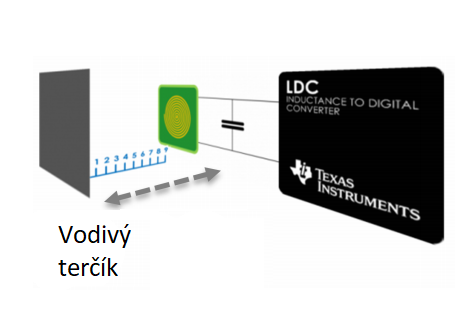
\includegraphics[width=200pt]{kapitoly/obrazky/E4/elektronika_tlakove_desky/civka_tercik_LDC.png}
    \caption{Schematické zobrazení cívky a~terčíku \parencite{LDC-cd1}}
    \label{fig:E4-sch_civka_tercik}
\end{figure}

\enlargethispage{5mm}
Pro snímání terčíku používám čip \href{https://www.ti.com/lit/ds/symlink/ldc1612.pdf?ts=1612018658531&ref_url=https%253A%252F%252Fwww.google.com%252F}{LDC1614} \parencite{LDC1614}
nebo \href{https://www.ti.com/lit/ds/symlink/ldc1312.pdf?ts=1612017390818&ref_url=https%253A%252F%252Fwww.google.com%252F}{LDC1314}, 
které se liší prakticky jen rozlišením. LDC1314 disponuje dvanáctibitovým AD převodníkem a~LDC1614 dvacetiosmibitovým AD převodníkem 
a~je tak schopen detekovat pohyb terčíku s~rozlišením až na 10 nm.

\begin{figure}[h]
    \centering
    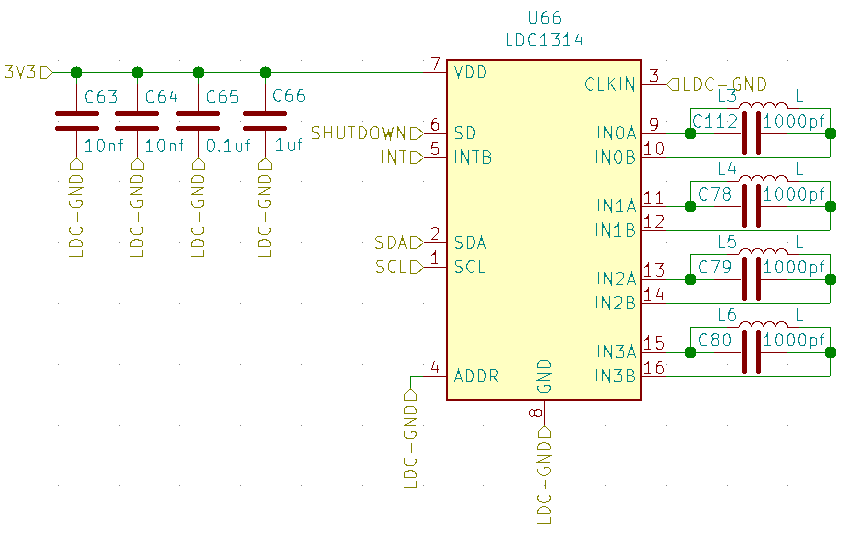
\includegraphics[width=\textwidth]{kapitoly/obrazky/E4/elektronika_tlakove_desky/moje_zapojeni.png}
    \caption{Zapojení čipu LDC1314 na desce trezoru}
    \label{fig:E4-LDC}
\end{figure}

Čip LDC komunikuje po sběrnici I2C, která umožňuje komunikaci jednoho mastera\footnote{Čip, který řídí komunikaci.} s~až 128 slavy.\footnote{Čipy, které přijímají příkazy od mastera a~pouze mu odpovídají.} LDC také umožňuje volbu ze dvou I2C adres, aby se dala adresa změnit v~případná 
kolize s~jiným čipem, který by měl stejnou adresu.\footnote{Např. aby se daly použít dva čipy LDC na jedné sběrnici I2C.}

Cívky použité na trezoru jsou vyrobeny jako reliéf ve vrstvě mědi přímo na DPS. Jejich vzhled jsem navrhoval v~simulátoru od firmy Texas Instruments, 
vytvořeném konkrétně pro LDC čipy, a~s~pomocí popisů reálných aplikací \parencite{LDC-cd0}, \parencite{LDC-cd1}, které firma Texas Instruments zveřejňuje.

% obrázek ze simulátoru

Výsledná cívka je vytvořena na dvouvrstvé desce a~na každé vrstvě má patnáct závitů s~drahou o~síle 0,152~mm se stejně velkou mezerou, 
vzhled je vidět na obrázku \obr{fig:E4-relief_civka}.

\enlargethispage{5mm}
Celý trezor obsahuje dvě samostatné elektronické desky, přičemž na jedné je osazen jen kruh z~LED WS2812 a~snímání tlakové desky, které zabírá 
většinu této desky což je vidět na obrázku \obr{fig:E4-LedDeska}.